\documentclass[12pt]{article}
%%%%%%begin preamble
\usepackage[hmargin=1in, vmargin=1in]{geometry} % Margins
\usepackage{hyperref}
\usepackage{url}
\usepackage[numbers]{natbib}
\usepackage{graphicx}
\usepackage{amsmath}
\usepackage{amsfonts}
\usepackage{amssymb}
\usepackage{wrapfig}

\usepackage{multicol}
\usepackage{etoolbox}
%\patchcmd{\thebibliography}{\section*{\refname}}
%    {\begin{multicols}{2}[\section*{\refname}]}{}{}
%\patchcmd{\endthebibliography}{\endlist}{\endlist\end{multicols}}{}{}


\usepackage[normalem]{ulem}
\usepackage{xcolor}
\newcommand{\edit}[2]{\textcolor{purple}{\sout{#1} \textbf{#2}}}

\hypersetup{
  colorlinks   = true,
  %citecolor    = blue
  citecolor    = blue
  % gray is not being found!?!
  % gray is found if pdfpages is used... crap.
  %citecolor    = grey
  %citecolor    = Gray
}


%% headers
\usepackage{fancyhdr}
\pagestyle{fancy}
\fancyhf{} % sets both header and footer to nothing
\lhead{Evan H. Anders}
\rhead{Research Statement}
\cfoot{\footnotesize{\thepage}}
%\pagestyle{empty}
%\pagenumbering{gobble}
%\renewcommand*{\thefootnote}{\fnsymbol{footnote}}

\renewcommand{\vec}{\ensuremath{\boldsymbol}}
\newcommand{\dedalus}{\href{http://dedalus-project.org}{Dedalus}}
\newcommand{\del}{\ensuremath{\vec{\nabla}}}
\newcommand{\scrS}{\ensuremath{\mathcal{S}}}

\newcommand{\prf}{PRF}
\newcommand{\prd}{PRD}
\newcommand{\prr}{PRR}
\newcommand{\ssr}{SSR}
\newcommand{\araa}{ARAA}
\newcommand{\mnras}{MNRAS}
\newcommand{\aap}{A\&A}
\newcommand{\apjl}{ApJL}
\newcommand{\apj}{ApJ}
\newcommand{\apjs}{ApJL}
\newcommand{\nat}{Nature}

\newcommand{\sct}[1]{\vspace{0.3cm}\hspace{-\parindent}\textbf{\underline{#1}}\hspace{0.3cm}}

%\newcommand{\nosection}[1]{%
%  \refstepcounter{section}%
%  \addcontentsline{toc}{section}{\protect\numberline{\thesection}#1}%
%  \markright{#1}}
%\newcommand{\nosubsection}[1]{%
%  \refstepcounter{subsection}%
%  \addcontentsline{toc}{subsection}{\protect\numberline{\thesubsection}#1}%
%  \markright{#1}}

%\usepackage{atbegshi}
%%%%%%end preamble


%Make bibliography 2col
\bibliographystyle{apj_small}
\makeatletter
\renewenvironment{thebibliography}[1]
     {\begin{multicols}{2}[\paragraph*{\refname}\vspace{-0.1in}]%
      \@mkboth{\MakeUppercase\refname}{\MakeUppercase\refname}%
      \list{\@biblabel{\@arabic\c@enumiv}}%
           {\settowidth\labelwidth{\@biblabel{#1}}%
            \leftmargin\labelwidth
            \advance\leftmargin\labelsep
            \@openbib@code
            \usecounter{enumiv}%
            \let\p@enumiv\@empty
            \renewcommand\theenumiv{\@arabic\c@enumiv}}%
      \setlength{\itemsep}{-2pt}
      \sloppy
      \clubpenalty4000
      \@clubpenalty \clubpenalty
      \widowpenalty4000%
      \sfcode`\.\@m}
     {\def\@noitemerr
       {\@latex@warning{Empty `thebibliography' environment}}%
      \endlist\end{multicols}}
\makeatother



\begin{document}
\thispagestyle{fancy}

\sct{Context \& Aims}
Kilometer scale ground-based gravitational wave observatories have revolutionized our ability to detect and characterize the compact remnants of stars.
These observatories like \emph{LIGO}, \emph{VIRGO}, and \emph{Kamioka} are expected to annually detect tens of compact object mergers, from which we will gain further understanding of the mass and spin distribution of these remnants \citep{roulet_etal_2021}.
This expanded understanding of the end stages of stellar evolution will provide constraints on high-precision stellar evolution models \citep{mesa6}, which are necessary for explaining the masses and spins we will observe.
In particular, nonlinear 3D magnetohydrodynamical processes like convection and dynamo-driven angular momentum transport are poorly modeled and understood in the context of stellar evolution.
Mixing at the convective core boundary of massive stars ($M_* \gtrsim 1.1 M_\odot$) leads to core mass uncertainties of up to 70\% \citep{kaiser_etal_2020}, making the evolutionary pathway of a star from birth to death unclear.
The manner in which differential rotation and magnetism interact to redistribute angular momentum in stellar interiors is also poorly understood, but current best models suggest that black holes born from single stars should spin slowly \citep{fuller_ma_2019}.
State-of-the-art 3D simulations are required to explore and calibrate new parameterizations of transport processes in 1D stellar evolution calculations.

\textbf{The goal of my research plan is to build a next-generation set of global and local 3D numerical simulations, which will answer the following questions:}\vspace{-0.2cm}
\begin{enumerate}
    \item How large are convective cores in massive stars? \vspace{-0.2cm}
    \item How efficiently do dynamos in stable radiative zones redistribute angular momentum?
\end{enumerate}

\sct{My Prior Research}
My research is rooted in fluid dynamics and inspired by observations of stars.
I use the \emph{Dedalus} \citep{burns_etal_2020} pseudospectral code to design and run state-of-the-art simulations which I use to learn about mixing processes like convection in stars.
\textbf{A core focus of my research has been to push the boundaries of \emph{time} evolution, while other studies have focused on \emph{spatial} resolution; my focus on the time domain has led to key discoveries in my career.}
When I was a graduate student, I focused on fundamental studies of convection.
I studied heat transport in compressible convection with  \citep{anders_etal_2019_rot} and without \citep{anders_brown_2017} rotation.
I studied how fast convection interacts with the slow evolution of the background thermal structure in convective regions \citep{anders_etal_2018,anders_etal_2020}; some dynamical snapshots from these studies are in shown the top two panels of Fig.~\ref{fig:past}.
I also studied convection at the smallest scales, examining individual downflows in the Sun's convection zone \cite{anders_etal_2019_thermals}.
As a postdoctoral fellow at Northwestern, I have connected my theoretical research with modern observational puzzles.
I have formed collaborations with observers and 1D modelers alike to understand what sets the position of a convective boundary \citep{anders_etal_2022b} (see Fig.~\ref{fig:past}, middle panels), and I have discovered the process that inflates the convective cores of stars relative to standard models \citep{anders_etal_2022a} (see Fig.~\ref{fig:past}, bottom panels).
I am now finishing a project focusing on gravity wave generation by core convection and the observable signals of these waves, for direct comparison with e.g., asteroseismic observations.

\begin{figure}
    \centering
    \vspace{-0.5cm}
    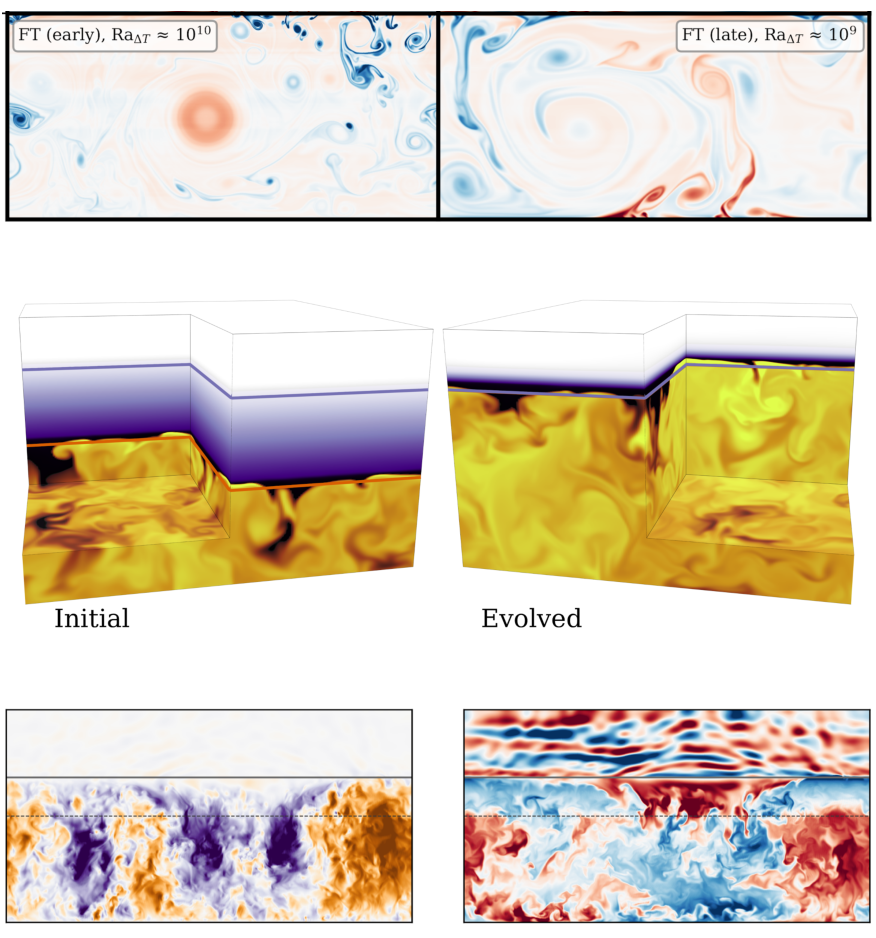
\includegraphics[width=\textwidth]{past_collage.pdf}
    \vspace{-1cm}
    \caption{(Top panels) Snapshots of the temperature anomaly in convective simulations at early (left) and late (right) times \citep{anders_etal_2020}.
    The disequilibrium early state demonstrates more turbulent flows and flow asymmetries than occur in the evolved, saturated state.
    \\
    (Middle panels) Snapshots of the composition field in a convective simulation at early (left) and late (right) times \citep{anders_etal_2022b}.
    The stable composition gradient (purple gradient) is entrained over time by overshooting convective motions into the well-mixed (yellow) convection zone.
    \\
    (Bottom panels) Snapshots of the vertical velocity (left) and temperature anomaly (right) at the same time in a simulation with convective penetration \citep{anders_etal_2022a}.
    In the left panel, we see broad upflows (orange) and downflows (purple).
    Upflows are hot (red) in the bulk convection zone but turn cold (blue) when they cross into the penetration zone (between the dashed line and solid line).
    \label{fig:past}
    }
\end{figure}


\newpage
\sct{Future Focus I: Convective Boundary Mixing}
Observations demonstrate a need for improved models of convective boundary mixing (CBM) \citep{johnston2021}.
For example, an unexplained mass-dependent CBM is required to reproduce observed eclipsing binary populations  \citep{claret_torres_2019}.
Asteroseismology allows us to directly probe near-core CBM, revealing extensive mixing occurs near convective core boundaries \citep{michielsen_etal_2019, pedersen_etal_2021}.
The amount of CBM used in a stellar evolution model modifies the evolution of a star's luminosity and effective temperature as well as the mass of the eventual remnant that it leaves behind \citep{castro_etal_2014,higgins_vink_2019}.


To understand the fluid dynamical picture behind CBM, I will create simulations of the cores of massive stars using the \emph{Dedalus} \citep{burns_etal_2020} code.
These simulations will differ from past simulations of massive stars, because they will include the full ``ball'' geometry of the convective core, they will employ the fully compressible equations without any luminosity boosting, and they will be relaxed into thermal equilibrium (See Fig.~\ref{fig:star} for a preliminary example of one of these simulations).
\emph{Dedalus} was recently updated with the state-of-the-art ability to simulate flows that pass through the coordinate singularity at $r = 0$ in spherical coordinates \citep{vasil_etal_2019,lecoanet_etal_2019}; most prior codes used a spherical shell geometry with a small interior ``cutout'' of the core.
Our implicit-explicit (IMEX) timestepping scheme allows us to circumvent timestepping restrictions from fast sound waves \citep{anders_brown_2017}, so we can take fast timesteps without boosting the luminosity as many prior simulations have done.
Evolving a simulation to thermal equilibration using classic timestepping techniques can take thousands of convective overturn timescales \citep{anders_etal_2022a,anders_etal_2022b}.
Fortunately, I have developed methods of ``accelerated evolution'' \citep{anders_etal_2018}, which self-consistently equilibrate simulations using an order of magnitude fewer cpu-hours than traditional timestepping.



\begin{wrapfigure}{r}{0.5\textwidth}
  \begin{center}
      \vspace{-1.6cm}
    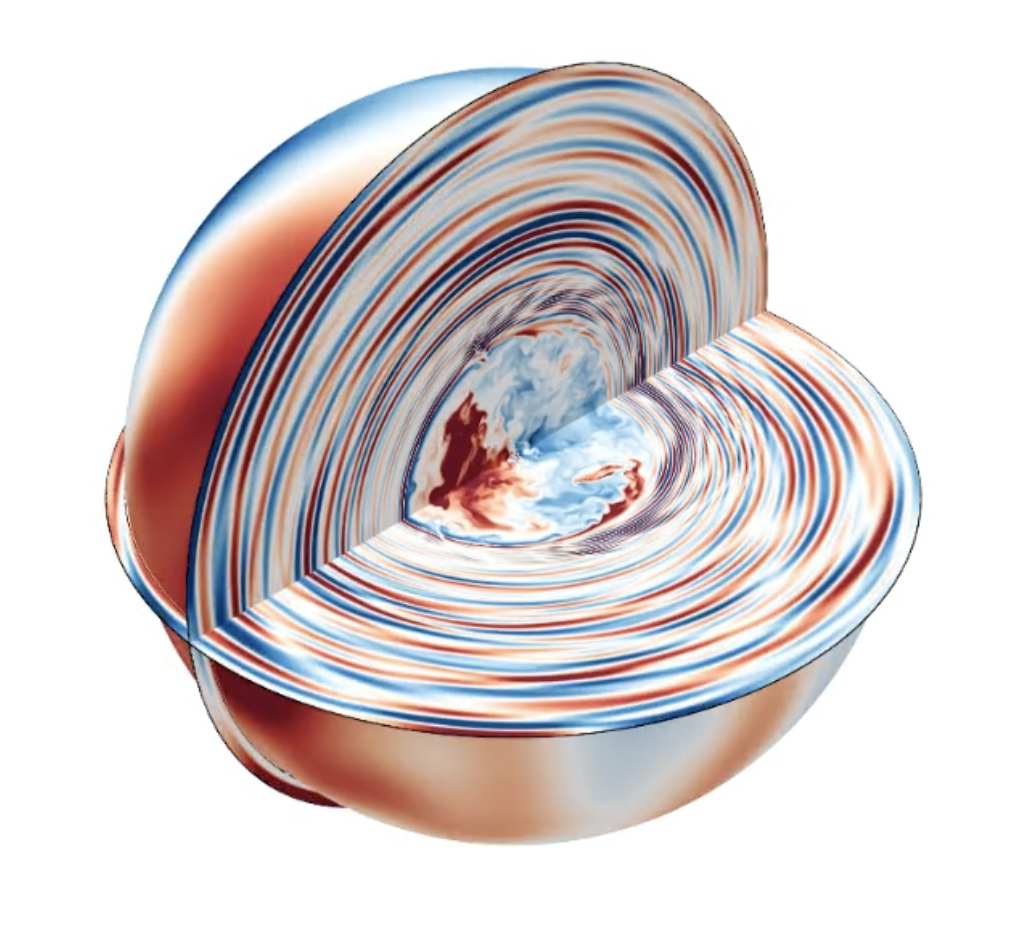
\includegraphics[width=0.45\textwidth]{dedalus_massive_star.png}
      \vspace{-1.3cm}
  \end{center}
    \caption{A simulation I ran in \emph{Dedalus} of a {$40 \,M_{\odot}$} star. 
    The entropy field is visualized; red is hot and buoyantly rises, blue is cold and falls. 
    We see a convective core with a strong dipole flow and an outer radiative envelope with internal gravity waves. \label{fig:star}}
    \vspace{-0.5cm}
\end{wrapfigure}
I will study CBM in fully compressible simulations whose background stratifications are based upon \emph{MESA} (Modules for Experiments in Stellar Astrophysics) models of massive stars.
I will study non-rotating and rotating stars with masses varying in the range $M_* = 1.1-40 M_{\odot}$ (the lowest masses where convective cores appear, up to high masses).
My results will calibrate a 1D implementation of convective boundary mixing, which I will then implement into the open-source \emph{MESA} software instrument.
Throughout this process, I will build my simulation code with ease-of-use for the user in mind, and this code will be made publicly available and citeable so that the community has access to a robust tool for studying fluid dynamics in massive stars.

\textbf{\underline{\emph{Deliverable:}} The first rotating, 3D simulations of core convection that include $\boldsymbol{r = 0}$ and reach thermal equilibrium.}

\newpage
\sct{Future Focus II: The Nonlinear Saturation of the Tayler Instability}
Modern asteroseismic measurements have revealed the nature of the internal rotation profiles of stars \citep{beck_etal_2012,saio_etal_2015,hermes_etal_2017}.
These observations reveal internal rotation rates which are much slower than expected, so some process must be efficiently redistributing angular momentum \citep{ji_etal_2022}.
The Tayler-Spruit (TS) Dynamo \citep{spruit2002} is frequently invoked as the likely mechanism which converts rotational energy into magnetic energy to redistribute angular momentum in the stable radiative interiors of stars.
Recently, Ref.~\citep{fuller_etal_2019} re-evaluated the efficiency of this mechanism and proposed compelling arguments for why the TS mechanism can efficiently slow the spins of stars.
The TS dynamo depends upon the Tayler instability, which distorts and twists toroidal magnetic fields \citep{spruit1999}.
While the linear Tayler instability is understood, the process which satures this instability and thus controls the angular momentum transport efficiency of the TS dynamo remains uncertain.

The Tayler instability in stars has a few important ingredients: an azimuthal magnetic field, global rotation, and a stable stratification.
Ref.~\citep{guerrero_etal_2019} simulated the instability without rotation and Ref.~\citep{weber_etal_2015} simulated the instability in the absence of a stable stratification.
Early studies by Ref.~\citep{braithwaite2006} included both of these effects but also included complications which made it difficult to achieve the scale separation required to resolve the Tayler instability.
Recently, Ref.~\citep{ji_etal_2022} studied the first simulations of the Tayler instability in the proper timescale regime which included all of these important ingredients.
While this simulation design could shed light on the saturation mechanism of the Tayler instability, these simulations could not achieve a sufficiently large separation of the various relevant timescales in the problem.
As a result, these simulations saturated because of a nonlinear shear mechanism which is not expected to operate in stellar interiors.
Additional complex simulations including all of the above ingredients plus differential rotation in spherical geometry have recently been reported \citep{petitdemange_etal_2022}, and the nonlinear saturation is claimed to mimick the one proposed by Spruit \citep{spruit2002}.
However, their simulation data show instabilities present that are not the Tayler instability, so it is difficult to understand how their results relate to the TS dynamo.

As a postdoctoral fellow at Carnegie, I will study the nonlinear saturation mechanisms of the Tayler instability.
I will first study the simplest possible relevant case: the Tayler instability subject to stable stratification but not subject to rotation.
While all massive stars rotate rapidly \citep{jermyn_etal_2022_atlas}, the inclusion of rotation introduces an additional timescale constraint which limits the relevant range of parameter space available to 3D simulations.
I will use my expertise in the methods used by the convection community \citep{ahlers_etal_2009,aurnou_etal_2020} to studying the force balances present during nonlinear saturation and to examine what drives dissipation.
Once I understand how the instability saturates in the absence of rotation, I will include rotation and understand how it changes what was learned in the non-rotating case.
I will re-evaluate the saturation arguments presented in Refs.~\citep{spruit2002,fuller_etal_2019} to determine if they are consistent with the fundamental mechanism at work in these simulations.
I will then update angular momentum prescriptions to appropriately incorporate the lessons we have learned, implement these prescriptions into the open-source \emph{MESA} stellar structure code, and understand how our updated understanding of the Tayler instability changes our theoretical view of the evolution of differential rotation in stellar interiors.

\textbf{\underline{\emph{Deliverable:}} A new prescription for angular momentum transport by the TS dynamo calibrated based on 3D magnetohydrodynamical simulations.}

\sct{Connections at Carnegie}
I would love to spend the next stage of my career at Carnegie, specifically the Carnegie Theoretical Astrophysics Center.
My research most naturally fits into the Stellar Evolution research topic, and I would be excited to collaborate with Dr.~Piro on the research proposed here.
I focus my work on the progenitors of compact objects which can now be observed through gravitational wave interferometers, and I hope also to plug in to the High Energy Astrophysics work at CTAC to learn more about constraints that gravitational wave astronomy places on my work.
I have always been interested in finding ways to apply my simulation techniques to modern problems in exoplanetary science, including questions of convective mixing in planetary atmospheres, and look forward to exploring research avenues in exoplanetary science.
Carnegie's computational resources (on the order of 1-2 million cpu-hours per year) is an excellent fit for my research plan, and will allow me to conduct most of the work proposed here.

I have used the extremely flexible \emph{Dedalus} code for eight years; outside of the five core developers, I am the leading Github contributor to the code base.
I know \emph{Dedalus} inside and out, and would be happy to provide support to any other members of Carnegie who are interested in using a flexible and general PDE solver like \emph{Dedalus} on their own research problems.
\emph{Dedalus} has been used to study a broad range of topics in astrophysics and outside of astrophysics (including e.g., quantum superfluids and the formation of bacterial sheets), and I hope to use my knowledge of \emph{Dedalus} to form collaborations outside of my current expertise in stellar interiors.

{\small%scriptsize
\bibliography{biblio}
}
\end{document}
